\chapter{Desarrollo}
\label{ch:desarrollo}


El hardware utilizado tiene las siguientes especificaciones:
\begin{itemize}
    \item CPU: AMD Ryzen 5 3600XT (12) @ 3.800
    \item GPU: AMD Radeon RX6800XT 
    \item RAM: 16GB CL16 @ 3000
    \item DISCO: SSD NVME 500GB
    \item SSOO: Linux 5.15.0-107-generic \#117~20.04.1-Ubuntu
\end{itemize}

El desarrollo fue realizado en Visual Studio Code, haciendo uso de Git y GitHub como sistema de control de versiones y copia de seguridad remota del desarrollo realizado.
El repositorio consta de la siguiente estructura de carpetas:

\begin{verbatim}
├── datasets/
│   └── CLEAN_REFIT_081116/
├── encoding
│   ├── REFIT_GAF/
│   │   ├── house1/
│   │   ...
│   │   ├── house21/
│   │   └── meta/
│   └── thSafe/
└── full_model
    ├── cspvenv/
    ├── data/
    │   └── REFIT_GAF -> /encoding/REFIT_GAF
    ├── first_test/
    └── src/

\end{verbatim}

\section{Planificación}
\label{sec:planificacion}
Se realizó dos tandas de organización y planificación de tareas. La primera al principio del semestre y la segunda a mediados de abril. 
Las dificultades en la planificación fueron una combinación de motivos externos y una perspectiva algo ingenua del tiempo a invertir y el ritmo de progreso.
Debido a la falta de conocimientos, se ha dedicado un tiempo considerable (unas 60-80 horas) a realizar investigación y estudio, para poder comprender las técnicas y modelos implementados el estado del arte.

En lo que respecta al desarrollo, se han dedicado unas 80-100 horas.

Los principales problemas fueron: la dificultad para programar un codificador en C++ y OpenCL, debido a la curva de dificultad que representa aprender un lenguaje para una nueva arquitectura y los retos que presenta la gran cantidad de datos usada para el entrenamiento de inteligencia artificial. 


\section{REFIT Dataset}
Tras una investigación de los potenicales datasets, se decidió usar como dataset REFIT. El nombre completo del dataset es \enquote{Personalised Retrofit Decision Support Tools For UK Homes Using Smart Home Technology}\autocite{REFIT}.
\subsection{Características principales}
Puede encontrarse todo el detalle sobre el dataset en el artículo publicado por David Murray, Lina Stankovic y Vladimir Stankovic \autocite{REFIT}.

El dataset recoge datos de 20 casas durante un periodo continuo de dos años, con un periodo de medición superior a un minuto entre mediciones para todas las casas. Siendo este el único dataset de Gran Bretaña con estas características.
Se miden 9 dispositivos además del consumo agregado. Todas las mediciones se realizaron en vatios. 

\begin{figure}[H]
    \centering
    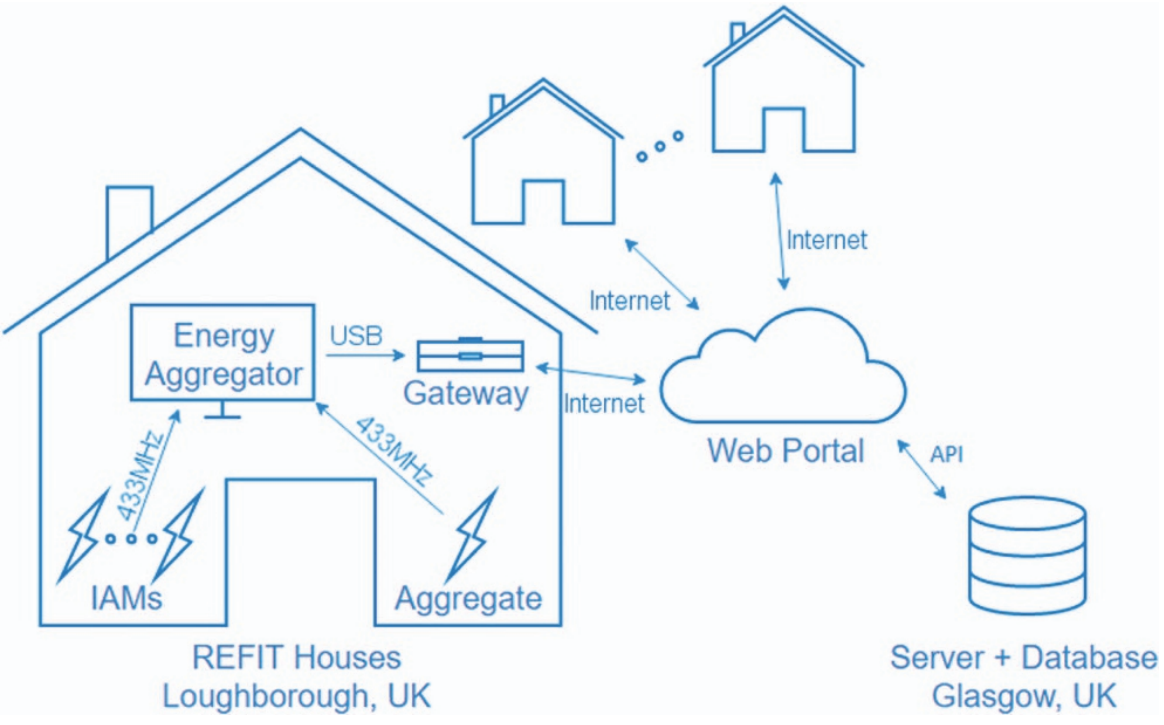
\includegraphics[height=250px]{images/REFITmodeloDatos.png}
    \caption{El modelo de recolección de datos (propiedad de \autocite{REFIT})}
    \label{diagramaBBDD}
\end{figure}

El dataset ocupa unos 5GB de memoria, se presentan todas las mediciones de una sola casa en archivos CSV. Siguiendo la distribución:
\begin{center}
    Time, Unix, Aggregate, Appliance1, ... , Appliance9, Issues
\end{center}
En total, hay 20 archivos en recogen datos, y un vigésimo primer archivo conteniendo los metadatos de cada casa. Estos metadatos se limitan a especificar el tipo de dispositivo asociado al dispositivo o \textit{Appliance} 
\todo[inline]{añadir unas líneas de una casa y una y sus metadatos}

En cuanto a la recogida de datos, se definió un periodo de recogida de datos de ocho segundos. Por tanto los datos se recogieron con un desplazamiento temporal. Esto quiere decir que los datos de los dispositivos y el agregado no coinciden exactamente en el tiempo, habiendo una diferencia de unos segundos entre dispositivo y dispositvo. El acumulado (o agregado) se calculaba antes de que finalizase el periodo de ocho segundos.


\subsection{Pros y contras del dataset}

Las ventajas de este dataset son, su longitud en el tiempo y la facilidad de empezar a hacer un uso de los mismos. Ya que se busca investigar sobre la viabilidad de un modelo que haga uso de clasificadores de imágenes, esto habilita la posibilidad de realizar un trabajo de fin de grado con este tema. 

Hay una serie de problemas conocidos sobre el dataset. En el artículo de David Murray \autocite{REFIT} se mencionan los siguientes:
\begin{itemize}
    \item Ocasionalmente los medidores de dispositivos reportaban consumos muy por encima de de la carga máxima para un dispositivo de uso doméstico. Estas medidas se eliminaron del dataset.
    \item Hubo problemas con la sincronización temporal de los medidores de dispositivos. Esto conlleva discrepancias entre el agregado y las mediciones.
    \item Las mediciones del acumulado en casas 3, 11 y 21 se vieron afectadas debido a que los domicilios contaban con paneles solares, y recablear para evitar afectar a las medidas del acumulado no era posible.
    \item En algunos casos, los valores entre acumulado y dispositivos no coinciden debido a que no se monitorizaron otras variables para ajustar estas medidas conforme el ángulo de fase o el voltaje por cargas inductivas o capacitivas.
\end{itemize}

Debido a falta de clasificación en los metadatos, las casas 12 y 13 no fueron utilizadas para el entrenamiento.

\section{Parseado de REFIT a MYSQL}
Como primer paso, se decidió parsear todos los datos a una base de datos, escogiendo MYSQL como plataforma, para tener una lógica de acceso que permitiese ordenar los datos para su codificación conforme a diferentes algoritmos (secuencial, k-means) para poder extraer la mayor cantidad de características sobre los dispositivos en diferentes marcos temporales.

\subsection{Inconvenientes}
La inserción de datos en la base de datos fue tremendamente lenta. Para insertar un CSV entero, se tardaba en el peor de los casos cerca de las 72h de inserción continuada.
En parte esto se debe a que se mantuvo durante un tiempo la configuración del servidor MYSQL \textit{out of the box} sin realizar ningún cambio.

Más adelante se investigó cómo poder optimizar las inserciones. La solución fue reducir el número de inserciones a la base de datos y aumentar el volumen de datos por inserción. Quinientas mediciones por INSERT redujeron drásticamente el tiempo necesario, de 3 días a unos 15 minutos.

\subsection{Modelo de la BBDD}
Para este paso del desarrollo, se decidió un modelo simple, imitando la presentación de los datos en el csv.
\begin{figure}[H]
    \centering
    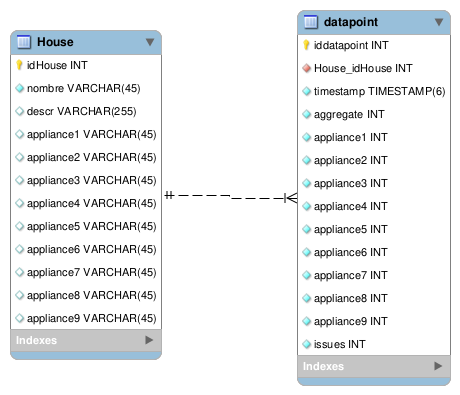
\includegraphics[height=250px]{images/db_parsingstep.png}
    \caption{El modelo de la BBDD en el parseo. Elaboración propia via MySQL Workbench}
    \label{diagramaBBDD}
\end{figure}

\subsection{Herramientas desarrolladas}
Para la inserción, se diseñaron dos programas en C++. Haciendo uso de la librería de conector de C++ a mysql. Se seleccionaba el archivo manualmente y comenzaba la inserción. 
Una vez iniciada la inserción de datos, esta se paraba en la misma fecha, el 31 de marzo. Esto se debía a que al insertar la fecha, habiendo un cambio de hora esa madrugada, las fechas no coincidían con las esperadas.

La solución a este problema fue desarrollar un programa que permitiese saltar a la línea donde daba el fallo, además de una serie de herramientas para \enquote{debuggear} la inserción de datos, pudiendo saltar a una línea específica e insertar manualmente o continuar la inserción.

Podemos observar el comportamiento de la herramienta, llamada sin argumentos:
\begin{lstlisting}[basicstyle=\ttfamily, backgroundcolor=\color{lightgray}]
    $ ./traversecsv 
    Usage: ./traversecsv <file> <house_id>
 \end{lstlisting}

Y llamada con argumentos
\begin{lstlisting}[basicstyle=\ttfamily, backgroundcolor=\color{lightgray}]
$ ./traversecsv CLEAN_REFIT_081116/CLEAN_House15.csv 15
    
Successfully connected to the database!
    Total lines in file: 6225697
    Press 'p' to print the next line 
        'i' to continue inserting 
        'j' to jump to a specific line 
        'r' to continue inserting until EOF
        's' to search for a line with a specific date
\end{lstlisting}

Además de desarrollar el programa, se cambió la configuración de fechas en el servidor MYSQL. 

\begin{lstlisting}[language=SQL,frame=ltrb,framesep=5pt,basicstyle=\normalsize,basicstyle=\ttfamily]
    SELECT @@global.time_zone, @@session.time_zone;
    SET GLOBAL time_zone = '+00:00';
    SET SESSION time_zone = '+00:00';
\end{lstlisting}

Este programa y su código fuente puede encontrarse a partir de la raíz del directorio dentro de \enquote{\textit{datasets/}}.

\section{Codificación GAF}
El método de codificación sigue una serie de pasos relativamente simples: 
\begin{lstlisting}
    (pseudocódigo)
    1. Dado un vector V de n elementos.
    for (n)
        V(n)=arccos(V(n))
        if V(n) > 1
            V(n)=1
        else if V(n) < -1
            V(n)=-1
    2. construimos la matriz M
    for (i)
        for (j)
            M=cos(V(i)+V(j))
\end{lstlisting}

\subsection{Primer Diseño}
Dado el volumen de los datos, se ideó un programa multihilo, con gestión asíncrona de llamadas y computación en GPU via kernels de OpenCL.

Se decidió separar el proceso de codificación en tres partes. Extracción de datos, Codificación de datos y Almacenamiento de Metadatos.

La extracción es altamente paralelizable. Consiste en extraer de la base de datos en bloques de un cierto tamaño y preparar series de datos para guardarlos en una estructura de datos accesible para los hilos posteriores. Se decidió por un hashmap thread safe.
Para notificar a los procesos de codificación las series que están listas para ser codificadas, se instanció una cola con mecanismos de sincronización para evitar posibles condiciones de carrera. Para reducir la redundancia de datos y el espacio de las estructuras de datos, sólo se introducen en la cola de series extraídas las claves resultantes de insertarlas en el hashmap.
Los hilos codificadores consumen claves de la cola de series extraídas, copiando las series del hashmap a un buffer y codificando el buffer. Se hace uso de un buffer por el mismo motivo que la extracción es en bloques de datos, para reducir el overhead de hacer una llamada de sistema. Una vez codificada una serie, se introduce de vuelta en el hashmap y se introduce su clave en la cola de series codificadas.
El Almacenamiento de metadatos copia el vector one-hot generado por el extractor y lo apenda a un archivo de texto. Las series codificadas siguen la misma convención para sus archivos. 

La motivación de gestionar las llamadas asíncronas debido a que el conector a la BBDD MYSQL las soportaba pero no daba más alternativas que la espera activa llevó al desarrollo de la clase \textit{EventLoop.hpp}. Se tomó prestado un concepto muy usado en servidores, en los que los sockets de un servidor (procesos individuales) traspasan sus peticiones a un proceso que se encarga de ejecutar las peticiones. Manteniendo así el coste de mantener una conexión con un servidor como un elemento separado de las operaciones del servicio. 
En el caso de la codificación, se implementó una solución de inserción de peticiones asíncronas, basado en promesas y futuros de funciones lambda que los procesos enviaban al EventLoop. Este se encargaba de recibirlas e instanciar un thread para ejecutar la petición, comprobando todas las peticiones de manera cíclica y devolviendo las promesas a los threads peticionantes (ver \ref{diagramaEventLoop}). 

\begin{figure}
    \centering
    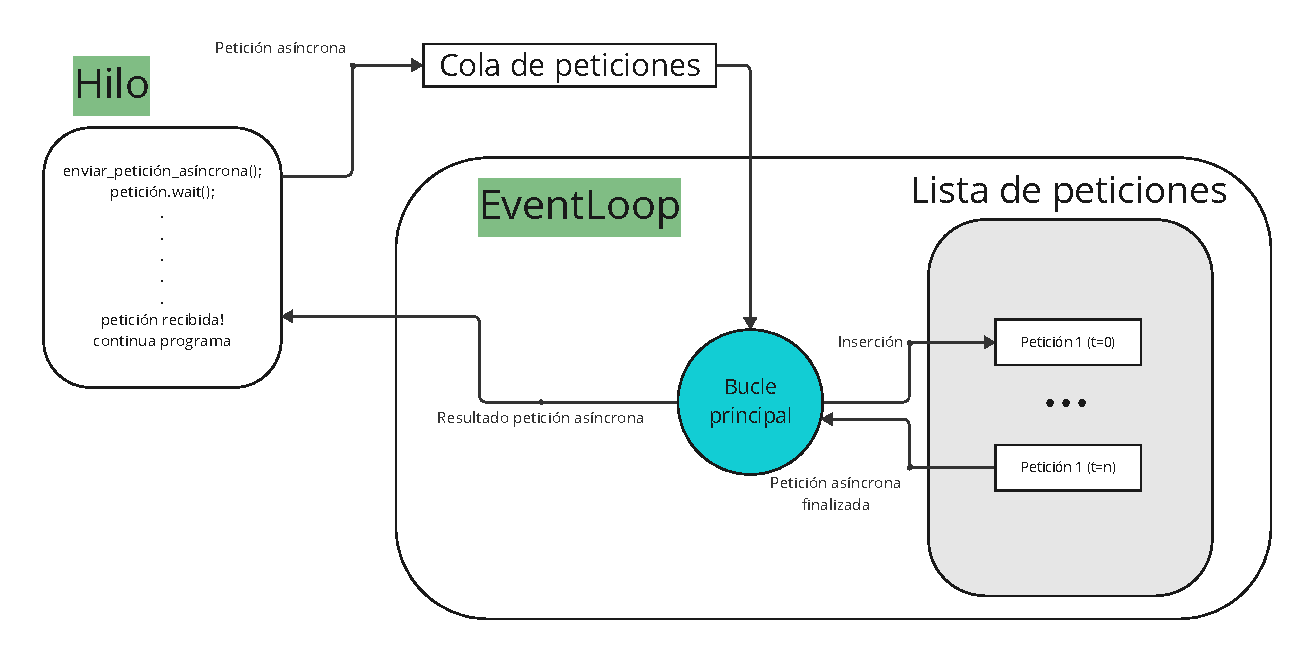
\includegraphics[height=250px]{images/EventLoop.pdf}
    \caption{Diseño abstracto del funcionamiento del EventLoop. Elaboración propia}
    \label{diagramaEventLoop}
\end{figure}

\subsection{Inconvenientes}
Este proceso de desarrollo se vio afectado por la optimización prematura. Sin embargo, se realizaron una serie de aprendizajes muy útiles en áreas que podrían beneficiar a futuro la escalabilidad de procesos como este en el campo de la inteligencia artificial.
\subsubsection{EventLoop}
Aún presentando una serie de ventajas a escala, la dificultad de devolver punteros sin desreferenciarlos fue el principal obstáculo de este sistema. Por lo que sólo se hizo un uso parcial de la solución desarrollada. 
\subsubsection{OpenCL}
Para la codificación de datos se intentó realizar un desarrollo de kernels en OpenCL que aprovechasen las ventajas de computación paralela de la GPU. Debido a una falta de experiencia en desarrollo en OpenCL y a la naturaleza temporal del trabajo, se debió de abandonar esta rama.

\subsection{Diseño Final}
Debido a los inconvenientes expuestos, el diseño final se hizo exclusivamente en la cpu, haciendo uso de openCV para construir las imágenes.

Se decidió instanciar tríos de hilos. 

Parámetros de invocación:
\begin{lstlisting}
$ ./host
Usage: 
./host <house number> <number of threads> <batch size> <number of batches>
SERIES SIZE IS A DEFINE
\end{lstlisting}
La última línea es un comentario relevante debido a que se consideró la posibilidad de alternar el tamaño de la serie y por ende el tamaño de las imágenes codificadas. 

Tiempo transcurrido en la codificación del los datos contenidos en \\ \textit{datasets/CLEAN\_REFIT\_081116/CLEAN\_House21.csv}.
\begin{lstlisting}
time ./host 22 7 21031 256

real	6m28,529s
user	38m35,273s
sys	1m52,445s
\end{lstlisting}

Este programa y su código fuente puede encontrarse a partir de la raíz del directorio dentro de \enquote{\textit{encoding/}}.

\section{Modelo y Entrenamiento}
\subsection{Modelo}
Se hace uso del modelo preentrenado CSPResNeXt50 de la librería timm por HuggingFace \autocite{crunchbase2023huggingface}.
Debido a la naturaleza multidimensional de los datos y a las predicciones deseadas del modelo, se requiere una serie de ajustes a la capa de entrada y a la de salida. Por lo tanto los pesos de esas dos capas serán perdidas.

El modelo CSPResNeXt50 es un modelo de clasificación de imágenes. El objetivo de este trabajo es aplicar transfer learning a un modelo ya preentrenado, para estudiar el rendimiento del modelo en un problema de clasificación de series temporales codificadas como imágenes.

Este modelo se basa en la arquitectura ResNeXt50, cuyas principales ventajas radican en la eficiencia de la red y el uso de la cardinalidad (dimensión extra) para aprender características más complejas, aumentando la precisión sin aumentar el ancho o profundidad de la red \autocite{xie2017aggregated}.
La arquitectura CSPNet se basa en la arquitectura ResNet, pero con la adición de un módulo CSP (Cross Stage Partial) que permite la fusión de características de diferentes etapas de la red, permitiendo una mejor generalización y aprendizaje de características más complejas \autocite{wang2019cspnet}.

Se decidió por un modelo multitarea. Ya que lo que muchos modelos no han alcanzado a realizar de forma exitosa es una clasificación de dispositivos eléctricos y una estimación del tiempo en el que se encuentran encendidos.

\begin{figure}[H]
    \centering
    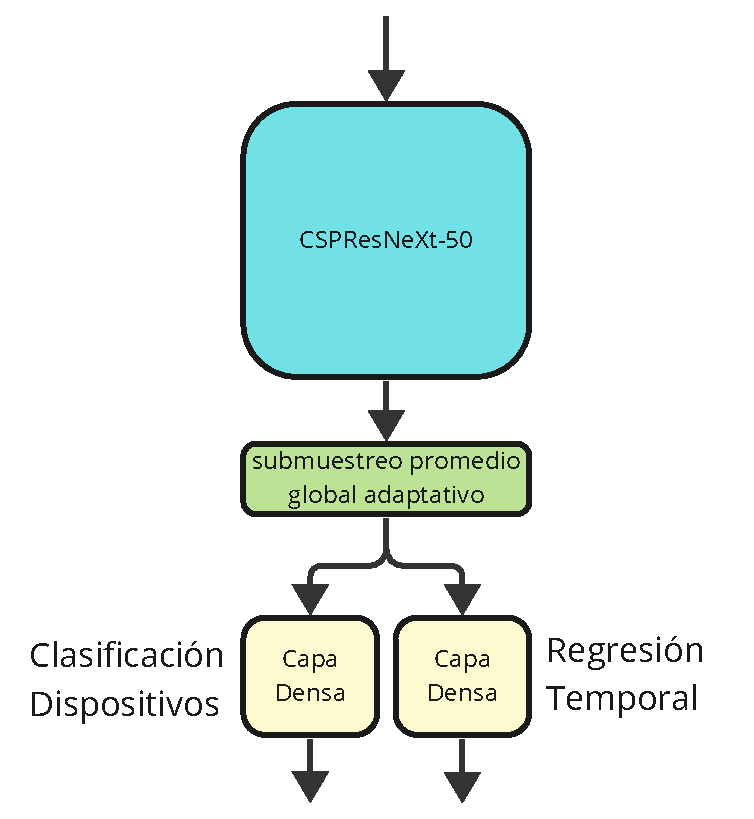
\includegraphics[height=250px]{images/modelo_IA.pdf}
    \caption{Diseño abstracto del modelo. Elaboración propia}
    \label{diagramaIA}
\end{figure}

Se extrae de la penúltima capa de CSPResNeXt50 los \textit{features} del modelo, introduciéndose a una capa de capa de submuestreo promedio global adaptativo. Esta capa es la entrada de nuestras dos capas de salida, dos capas densas que realizan la estimación de clases y estimación temporal (ver \ref{diagramaIA}).
Estos datos son dos vectores de 23 elementos cada uno. El primero es un vector one-hot y el segundo es un vector de valores enteros que representan el número de instancias de cada clase en la imagen.

\subsection{Pytorch}
Debido a que el único modelo que se encontró que cumplía los requisitos (modelo preentrenado, clasificación de imágenes, enfoque CSPNet) fue el modelo CSPResNeXt50, se decidió hacer uso de la librería Pytorch para el entrenamiento del modelo, ya que el modelo preentrenado se encontraba en la librería timm de HuggingFace.
Los modelos con enfoque CSPNet están fuertemente relacionados con la clasificación de imágenes que hacen uso de capas especializadas para la extracción de características que no resultan ventajosas para la tarea en cuestión. Por lo que la mayoría de modelos requerían una serie de modificaciones que salían del alcance del proyecto.

Para entrenar el modelo se hizo uso de la librería Pytorch, que permite el uso de la GPU para el entrenamiento de modelos de aprendizaje profundo.
Para esto, se instaló el módulo ROCm de Pytorch, que permite el uso de las GPU de AMD. Y la librería de Pytorch compatible con ROCm

El proceso de entrenamiento escogido fue el de desarrollar un script que implementa el dataloader de pytorch para cargar las imágenes codificadas y sus etiquetas. Y el desarrollo de un script que realiza las modificaciones necesarias al modelo para poder cumplir los requisitos de la tarea.  

En cuanto a los datos, tanto los vectores como la predicción temporal se expandieron a 23 elementos (las 23 clases del dataset). Los vectores temporales se normalizaron, mientras que el vector de clases no se normalizó.

\subsection{Entrenamiento}
Se desarrolló un script de entrenamiento. Los parámetros escogidos fueron los siguientes:
\begin{itemize}
    \item Número de épocas: 31
    \item Tamaño del lote: 20
    \item Learning rate: 0.001
    \item Optimizador: Adam
    \item Función de pérdida 1: CrossEntropyLoss
    \item Función de pérdida 2: MSELoss
\end{itemize}

El entrenamiento se realizó en una GPU AMD Radeon RX6800XT. El tiempo de entrenamiento fue de en torno a las 22 horas para las 31 épocas.

\subsubsection{Cálculo de Error}
Se decidieron por dos funciones de pérdida. La primera, la función de error con Entropía cruzada. Para la clasificación de los dispositivos eléctricos. Esta función de entropía penaliza solo las predicciones correctas, calculando el error sólo para predicciones correctas.
$$
CE=-\sum_{j=1}^{n}sum_{i=1}^{n} y_{i}\log{\hat{y_{i}}} \quad \text{\autocite{mao2023crossentropy}}
$$

Para implementar una función de pérdida de entropía cruzada personalizada, se aplica la función log-softmax a las predicciones. La función log-softmax se define como:

\[
\hat{y}_{\text{pred},ij} = \log \left( \frac{\exp(y_{\text{pred},ij})}{\sum_{k=1}^{C} \exp(y_{\text{pred},ik})} \right)
\]

donde \( y_{\text{pred},ij} \) es el logit predicho para la instancia \( i \) y la clase \( j \), y \( C \) es el número de clases.

A continuación, se calcula el producto elemento por elemento de las etiquetas verdaderas y las predicciones log-softmax:

\[
\text{E}_i = -\sum_{j=1}^{C} y_{\text{true},ij} \cdot \hat{y}_{\text{pred},ij}
\]

donde \( y_{\text{true},ij} \) es la etiqueta verdadera para la instancia \( i \) y la clase \( j \).

Luego, se suman las pérdidas a través de todas las clases para cada instancia:

\[
\text{E}_i = -\sum_{j=1}^{C} y_{\text{true},ij} \cdot \log \left( \frac{\exp(y_{\text{pred},ij})}{\sum_{k=1}^{C} \exp(y_{\text{pred},ik})} \right)
\]

Finalmente, se calcula la media de la pérdida a través de todas las instancias en el lote:

\[
\text{E} = \frac{1}{N} \sum_{i=1}^{N} \text{E}_i
\]

donde \( N \) es el número de instancias en el lote.

Combinando estos pasos, la expresión final para la función de pérdida de entropía cruzada personalizada es:

\[
\text{E} = -\frac{1}{N} \sum_{i=1}^{N} \sum_{j=1}^{C} y_{\text{true},ij} \cdot \log \left( \frac{\exp(y_{\text{pred},ij})}{\sum_{k=1}^{C} \exp(y_{\text{pred},ik})} \right)
\]

En python la implementación es la siguiente: 
\begin{lstlisting}[language=python]
import torch
import torch.nn as nn
import torch.nn.functional as F

class CustomCrossEntropyLoss(nn.Module):
        super(CustomCrossEntropyLoss, self).__init__()
    
    def forward(self, y_pred, y_true):
        y_pred = F.log_softmax(y_pred, dim=1)
        loss = -torch.sum(y_true * y_pred, dim=1)
        return loss.mean()
\end{lstlisting}

Para el segundo error, la regresión temporal de los tiempos en los que se encuentran encendidos los dispositivos eléctricos. Se escogió el error cuadrático medio.

Al hacer uso de dos funciones de error, y tener salidas diferentes para el modelo, se establece un equilibrado de pérdidas, sólo durante el periodo de entrenamiento.

Se decidió por un equilibrado de pérdidas con pesos basados en los gradientes de clases y tiempo. Se extraen los gradientes de la penúltima capa del modelo. Se normalizan y establecen los pesos como: 

$$
\text{peso}_k={(\frac{\text{grad norm}_k}{\frac{1}{N}\sum_{i=1}^{N}\text{grad norm}_i})}^\alpha
$$

Donde $\alpha$ es un hiperparámetro que controla la sensitividad del ajuste de los pesos.
Por último, se normalizan los pesos para que no se desestabilice la función total de pérdida.

Puede observarse el código en python asociado:
\begin{lstlisting}[language=python]
def calculate_loss(model, pred_class_count, pred_time, 
        true_class_count, true_time, training, alpha=1):
# Compute the losses
class_loss = CustomCrossEntropyLoss()(pred_class_count, true_class_count)
time_loss = F.mse_loss(pred_time, true_time)

if training:
    # Zero out any existing gradients
    model.zero_grad()

    # Calculate gradients for class_loss
    class_loss.backward(retain_graph=True)
    class_grads = [p.grad.clone().detach() for p in model.parameters()
            if p.grad is not None]
    class_grad_norm = torch.sqrt(sum([g.norm() ** 2 for g in class_grads]))

    # Zero gradients before calculating for the next loss
    model.zero_grad()

    # Calculate gradients for time_loss
    time_loss.backward(retain_graph=True)
    time_grads = [p.grad.clone().detach() for p in model.parameters() 
            if p.grad is not None]
    time_grad_norm = torch.sqrt(sum([g.norm() ** 2 for g in time_grads]))

    avg_grad_norm = (class_grad_norm + time_grad_norm) / 2
    class_weight = (class_grad_norm / avg_grad_norm).pow(alpha)
    time_weight = (time_grad_norm / avg_grad_norm).pow(alpha)

    sum_weights = class_weight + time_weight
    class_weight /= sum_weights
    time_weight /= sum_weights

    loss = class_loss * class_weight + time_loss * time_weight
else:
    loss = class_loss + time_loss

    return loss
\end{lstlisting}

\subsection{Inconvenientes}
El entrenamiento del modelo se vio afectado por la falta de experiencia en el uso de Pytorch y la falta de tiempo para investigar y aprender sobre la librería. Sin embargo, se logró realizar un entrenamiento exitoso del modelo.

Los principales inconvenientes que presenta el modelo se deben al tamaño de la red preentrenada. Es muy grande y podría beneficiarse de una reducción de tamaño. Además, el modelo CSPResNeXt50 no es el más ligero, por lo que el entrenamiento del modelo es lento y requiere de una GPU potente para poder realizarlo en un tiempo razonable.

Debido al hardware disponible, la GPU requirió de una serie de ajustes (undervolt, limitación de potencia y regulación de relojes) que limitaron el número de épocas y el tamaño de lote que podían realizarse en un tiempo razonable.

La validación del modelo no pudo implementarse eficientemente (alternando entre entrenamiento y validación para cada una de las épocas).

Los modelos multifuncionales son complejos de crear, entrenar y validar, este modelo no se ha mantenido exento de esos retos. Especialmente para alguien con poca o ninguna experiencia.
